
%\documentclass[calculator,allquestions,datasheet,mock,solutions]{exam_newMarcus2}
\documentclass[calculator,allquestions,datasheet,mock,Pens]{exam_newMarcus2}

% The full list of class options are
% calculator : Allows approved calculator use.
% datasheet : Adds a note that data sheet are attached to the exam.
% handbook : Allows the use of the engineering handbook.
% resit : Adds the resit markings to the paper.
% sample : Adds conspicuous SAMPLE markings to the paper
% solutions : Uses the contents of \solution commands (and \solmarks) to generate a solution file
% mock: For a mock-exam paper

\usepackage{pdfpages}  
\usepackage{lscape,comment} 
 
\coursecode{EX3029}%%
\coursetitle{Chemical Thermodynamics}
 
\examtime{14.00--16.00}%
\examdate{16}{11}{2017}% 
\examformat{Attempt ALL questions. \\ Each question is worth 20 marks.}

\newcommand{\frc}{\displaystyle\frac}
\newcommand{\br}[1]{\!\left( #1 \right)}
\newcommand{\abs}[1]{\left| #1 \right|}
\newcommand{\fracd}[2]{\frac{\mathrm{d} #1}{\mathrm{d} #2}}
\newcommand{\fracp}[2]{\frac{\partial #1}{\partial #2}}
\renewcommand{\d}[1]{\mathrm{d} #1 } 
\newcommand{\Ma}{\mathrm{M\!a}} 
\newcommand{\Partial}[3][error]{\left(\frc{\partial #1}{\partial #2}\right)_{#3}}
\newcommand{\mfr}[3][error]{#1_{#2}^{\left(#3\right)}} 



\begin{document}


%%%
%%% Question 01
%%%
\begin{question}

\end{question}

\clearpage




%%%
%%% Question 02
%%%
\begin{question}

\end{question} 
\clearpage


%%%
%%% Question 03 
%%%
\begin{question}
%
\end{question}

\clearpage


%%%
%%% Question 04
%%%
\begin{question}
  
\end{question}

\clearpage


%%%
%%% Question 05 
%%%
\begin{question}
  
\end{question}


\vfill
\paperend



\vfill 



%\begin{comment}
{
  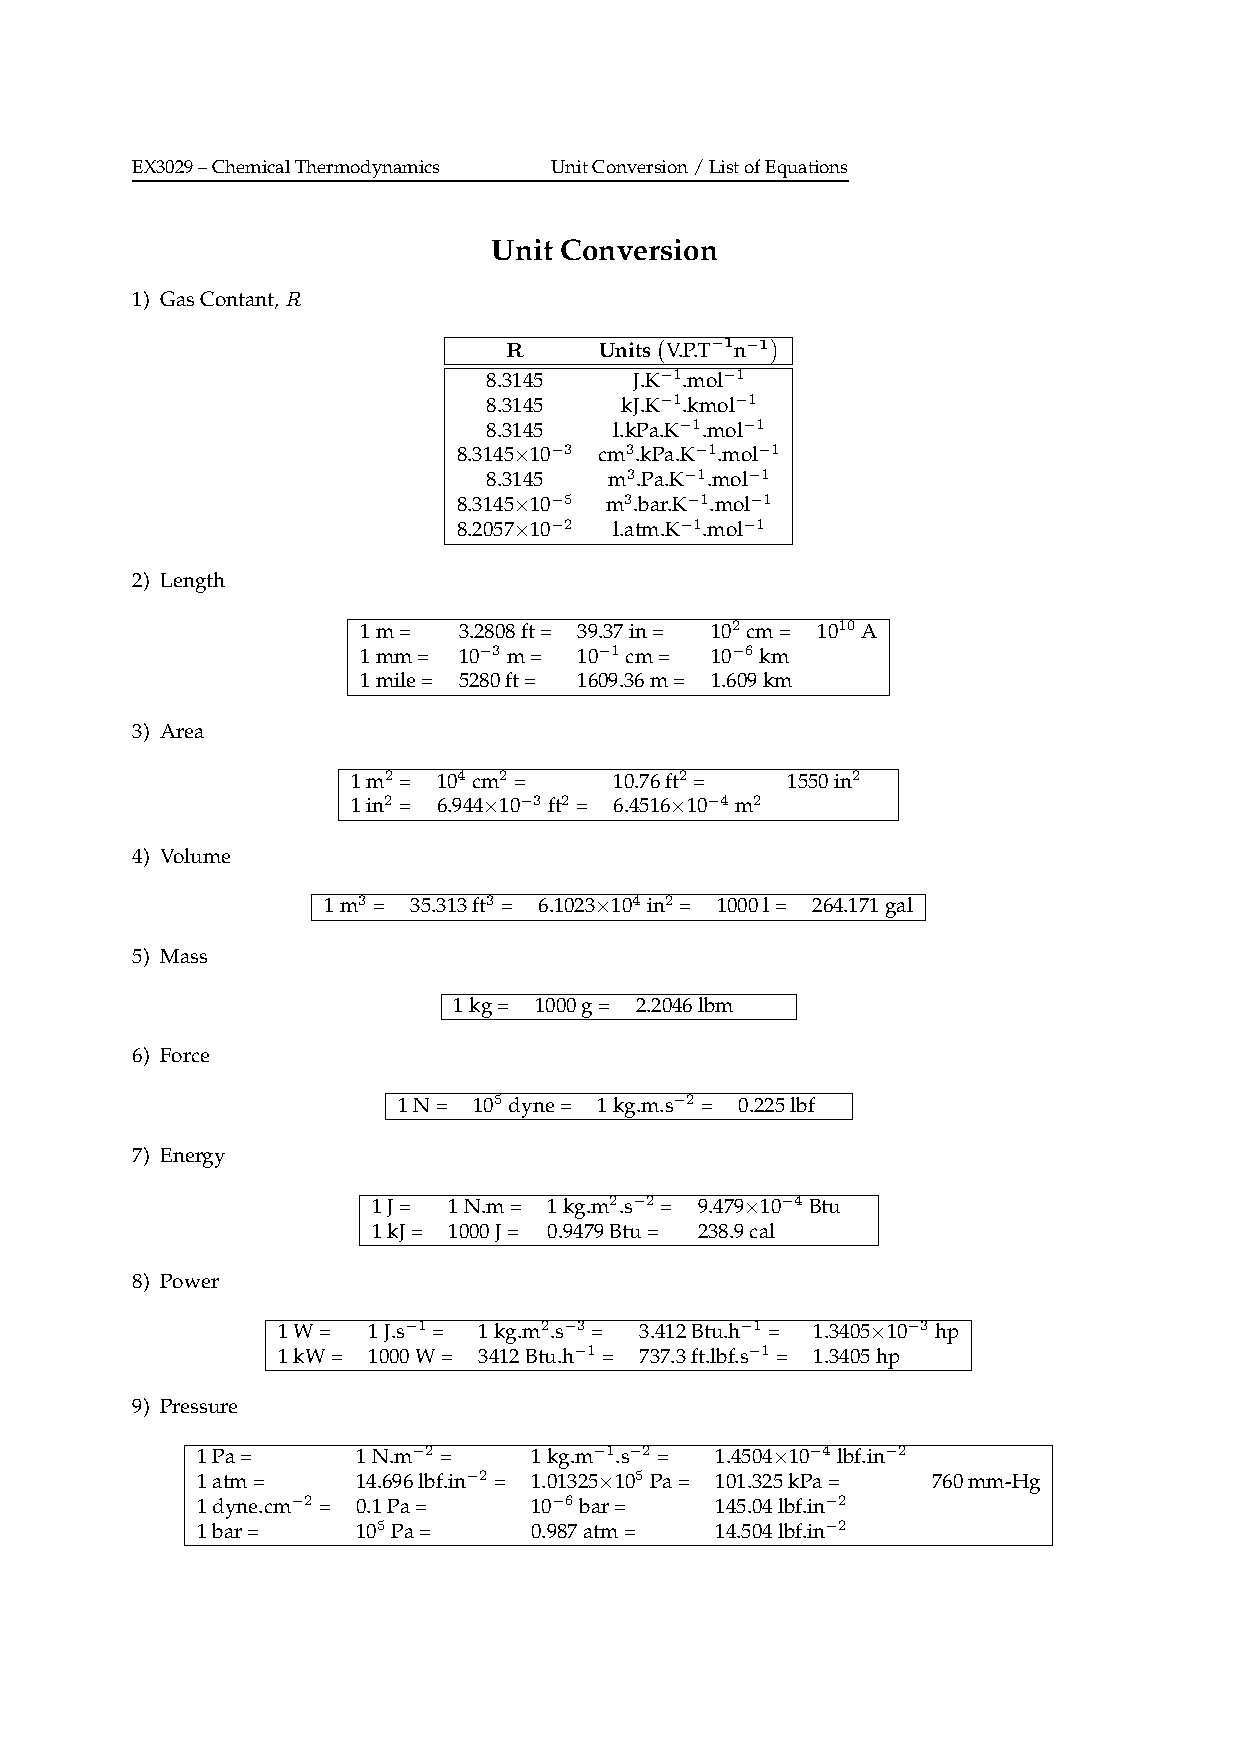
\includepdf[pages=-,fitpaper]{./Pics/EquationsList}
}
%\end{comment}



\end{document}
